
\begin{comment}
La entrada de wikipedia es una traducción literal del estándar 9126, ojalá
no se entienda como plagio. No sé si dejar los 
\end{comment}

\begin{description}

  \item[Functionality] Un conjunto de atributos que se relacionan con la 
existencia de un conjunto de funciones y sus propiedades específicas. 
Las funciones son aquellas que satisfacen las necesidades 
implícitas o explícitas

\SpecialItem
	\begin{description}
  		\item	 [Suitability:]  Atributos del software relacionados con la 
presencia y aptitud de un conjunto de funciones para tareas especificadas
  		\item[Accurateness:] Atributos del software relacionados con 
la disposición de resultados o efectos correctos o acordados
  		\item[Interoperability:] Atributos del software que se relacionan 
con su habilidad para la interacción con sistemas especificados.
  		\item[Compliance:]  Where appropriate certain industry (or government) 
laws and guidelines need to be complied with, i.e. SOX. This subcharacteristic 
addresses the compliant capability of software
  		\item[Security:] Atributos del software relacionados con su 
habilidad para prevenir acceso no autorizado ya sea accidental o 
deliberado, a programas y datos.
	\end{description}
	
  \item[Reliability] Un conjunto de atributos relacionados con la capacidad 
del software de mantener su nivel de prestación bajo condiciones
 establecidas durante un período establecido
	\SpecialItem
	\begin{description}
  		\item[Maturity:]  Atributos del software que se relacionan 
con la frecuencia de falla por fallas en el software
  		\item[Fault Tolerance:] Atributos del software que se relacionan 
con su habilidad para mantener un nivel especificado de desempeño en 
casos de fallas de software o de una infracción a su interfaz especificada
  		\item[Recoverability:] Atributos del software que se relacionan 
con la capacidad para restablecer su nivel de desempeño y recuperar 
los datos directamente afectos en caso de falla y en el tiempo y 
esfuerzo relacionado para ello.
  		\item[Reliability Compliance:]  La capacidad del producto 
software para adherirse a normas, convenciones o legislación 
relacionadas con la fiabilidad	
	\end{description}

  \item[Usability] Un conjunto de atributos relacionados con el esfuerzo 
necesario para su uso, y en la valoración individual de tal uso, por 
un establecido o implicado conjunto de usuarios
	\SpecialItem
	\begin{description}
  		\item[Understandability:] Atributos del software que se 
relacionan al esfuerzo de los usuarios para reconocer el 
concepto lógico y sus aplicaciones.
  		\item[Learnability:] Atributos del software que se relacionan 
al esfuerzo de los usuarios para reconocer el concepto lógico 
y sus aplicaciones.
  		\item[Operability:] Atributos del software que se relacionan 
con el esfuerzo de los usuario para la operación 
y control del software.
  		\item[Attractiveness:] FALTA OJO
		\item[Usability Compliance:]  FALTA OJO
	\end{description}
	
  \item[Efficiency] Conjunto de atributos relacionados con la relación 
entre el nivel de desempeño del software y la cantidad de 
recursos necesitados bajo condiciones establecidas.
	\SpecialItem
	\begin{description}
  		\item[Time Behaviour:] Atributos del software que se 
relacionan con los tiempos de respuesta y procesamiento y en las 
tasas de rendimientos en desempeñar su función.
  		\item[Resource Utilization:] Atributos del software que se relacionan 
al esfuerzo de los usuarios para reconocer el concepto lógico 
y sus aplicaciones.
  		\item[Efficiency Compliance:] Usar las cantidades y tipos de 
recursos adecuados cuando el software lleva a cabo su función bajo 
condiciones determinadas
	\end{description}
	
  \item[Maintainability] Conjunto de atributos relacionados con la 
facilidad de extender, modificar o corregir errores en un sistema 
software.
	\SpecialItem
	\begin{description}
  		\item[Analyzability:] Atributos del software relacionados con 
el esfuerzo necesario para el diagnóstico de deficiencias o causas 
de fallos, o identificaciones de partes a modificar.
  		\item[Changeability:] Atributos del software relacionados 
con el esfuerzo necesario para la modificación, corrección de falla, 
o cambio de ambiente.
  		\item[Stability:] Usar las cantidades y tipos de 
recursos adecuados cuando el software lleva a cabo su función bajo 
condiciones determinadas
		\item[Testability:] Atributos del software relacionados con 
el esfuerzo necesario para validar el software modificado.
		\item[Maintainability Compliance:] FALTA OJO
	\end{description}
	
  \item[Portability] Conjunto de atributos relacionados con la 
capacidad de un sistema software para ser transferido desde un
ambiente a otro.
	\SpecialItem
	\begin{description}
  		\item[Adaptability:] Atributos del software relacionados 
con la oportunidad para su adaptación a diferentes ambientes 
especificados sin aplicar otras acciones o medios que los 
proporcionados para este propósito por el software considerado.
  		\item[Installability:] Atributos del software relacionados con 
el esfuerzo necesario para instalar el software en un 
ambiente especificado.
  		\item[Co-Existence:] Coexistir con otro software 
independiente, en un entorno común, compartiendo 
recursos comunes.
		\item[Replaceability:] Atributos del software relacionados 
con la oportunidad y esfuerzo de usar el software en lugar de otro 
software especificado en el ambiente de dicho software 
especificado.
		\item[Portability Compliance:] Similar to compliance for 
functionality, but this characteristic relates to portability. 
One example would be Open SQL conformance which relates 
to portability of database used.
	\end{description}
\end{description}

%%%%%%%%%%%%%%%
%%%%%%%%%%%%%%


\bigskip
\begin{table}
\centering
\caption{Principales palabras claves y su significado} 
\begin{tabularx}{\textwidth}{p{4cm} X} 
\toprule[0.5pt]
	Model,Scheme,Protocol		&	El estudio propone algún modelo, esquema o protocolo	\\
	Security, Usability, Efficiency
	Reliabilty, Fault-Tolerance	&	El estudio se enfoca en alguno(as) de estas 
								características o sub-características tanto explicita 
								como implicitamente 	\\	
	Organisations				&	El estudio se enfoca en la relación entre los sistemas
								electrónicos y las organizaciones, tales como gobiernos
								y corporaciones.	\\
	Implementation			&	El estudio presenta resultados de alguna implementación \\
	Experience-Report			&	El estudio presenta resultados de algo \\
	Analysis					&	El estudio presenta sólo análisis y/o comparaciones de 
								algunos modelos,esquemas o protocolos. \\
	Formal definition			&	El estudio se enfoca en definir formalmente aspectos de
								sistemas, o de evaluarlos. \\
	Large-Scale,Small-Scale		&	El estudio se enfoca específicamente en votaciones de 
								determinado tamaño	\\
	System					&	El estudio propone un sistema completo de votación electrónica. \\
					
\bottomrule[0.5pt]
\end {tabularx}
\end{table}

%%%%%%%%%%%%%%%%%%%
%%%%%%%%%%%%%%%%%%


El esquema final de clasificación de los estudios en el mapeo 
sistemático pertenecen a 3 ejes:

\begin{itemize}
	\item \textbf{Temporal:} Marco de referencia temporal de los últimos 10 años, 2003-2013.
	\item \textbf{Requerimientos no funcionales:} Subconjunto de los requerimientos no funcionales
	dada su definición en el estándar 9126:2001, considerados a partir del trabajo de "falta cita"
	que considera estos como los más importantes.
	\item \textbf{Líneas de trabajo:} Etapas del
\end{itemize}


%%%
%%%%%%%%%%%%%%%%%%%
%%%%%%%%%%%%%%%%%%
%%%%%%%%%%%%%%%%%%%
%%%%%%%%%%%%%%%%%%

\begin{table}
\centering
\renewcommand{\arraystretch}{1}
\caption{Características y subcaracterísticas ISO/IEC 9126:2001}
\label{tab:esquema-clasificacion}
\begin{tabularx}{0.6\textwidth}{p{3cm} X} 
\toprule[1.5pt]
	\bf 	Característica		& 	\bf 	Subcaracterísticas  	\\
	Functionality			& 	Suitability	\\			 											
						&	Accurateness  		\\
						&	Interoperability 	\\
						&	Compliance 		\\
						&	Security 			\\ \hline
	Reliability				&	Maturity \\
						& 	Fault Tolerance \\
						&	Recoverability \\
						&	Reliability Compliance \\ \hline
	Usability				&	Understandability \\
						&	Learnability \\
						&	Operability \\
						&	Attractiveness \\
						&	Usability Compliance \\ \hline
	Efficiency				&	Time Behaviour \\
						&	Resource Utilization \\
						&	Efficiency Compliance \\ \hline
	Maintainability 			&	Analyzability \\
						&	Changeability \\
						&	Stability \\
						&	Testability \\
						&	Maintainability Compliance \\ \hline
	Portability 			&	Adaptability \\
						&	Installability \\
						&	Co-Existence \\
						&	Replaceability \\
						&	Portability Compliance \\
						
			
\bottomrule[0.5pt]
\end{tabularx}
\end{table}

%%%%%
% no mostrar los encabezados de capítulo, ademas de quitar espacio anterior %
\makeatletter
\def\@makechapterhead#1{%
  %\vspace*{\z@}%
  {\parindent \z@ \raggedright \normalfont
    \interlinepenalty\@M
    \Huge\bfseries  \thechapter.\quad #1\par\nobreak
    \vskip 22\p@
    \clearpage
  }}
\makeatother


%%%%%%%%%%%%%%
RECOMENDACION
	
	\item Construir protocolos que satisfagan requisitos de seguridad y que al mismo tiempo busquen eficiencia y 
		confiabilidad. Muchas propuestas de sistemas de votación electrónica se enfocan exclusivamente en lograr
		máxima seguridad, descuidando la escalabilidad del sistema cuando se utiliza a gran escala. Dado que el 
		alcance de las propuestas usualmente no incluye la implementación, 
		

		
		asumen que la implementa
		
		
		Varios modelos
		sencillamente omiten determinar la eficiencia de la propuesta, aunque es cierto que actualmente se necesitan
		de sistemas que resuelvan problemas de seguridad, la cantidad de vectores de ataque de 
		
		
		How anyone comes to this presumption is a mystery to me. Is there any version of any operating system 
		anywhere where the last security bug was found and fixed? Is there a major piece of software 
		anywhere that has been, and continues to be, vulnerability-free?
		
		Voting is as much a perception issue as it is a technological issue. It's not enough for the result to be
		mathematically accurate; every citizen must also be confident that it is correct. Around the world, 
		people protest or riot after an election not when their candidate loses, but when they think their candidate 
		lost unfairly. It is vital for a democracy that an election both accurately determine 
		the winner and adequately convince the loser.

%%%%

\begin{comment}


% formato de encabezados y pie de pagina


%\def \titulotesis {Identificación y evaluación de requerimientos no funcionales en modelos y aplicaciones de votación electrónica: un mapeo sistemático}







\end{comment}





%%%%%%%%%%%%%%%


\begin{comment}
%\end{comment}




%%%%%%%%%%%%%%%%%%%%%%%%%%%%%%%%%%%%%%%%%%

	\begin{itemize}

			\item \textbf{Requerimientos:}Han existido varios esfuerzos por establecer los requerimientos funcionales
				y no funcionales de los sistemas de votación electrónica \cite{Langer2010,Pesado2005}. 
				Los autores coinciden en que actualmente no existe un acuerdo preciso en la comunidad 
				acerca de todos los requerimientos de software que los sistemas de votación
				deben cumplir, ya que si bien los conceptos fundamentales están claros en los
				detalles es donde existe la mayor complejidad. \cite{Ikonomopoulos} identificó que 
				existe una necesidad para producir un conjunto de requerimientos sistemáticamente
				a partir de la regulación legal europea existente, en conjunto con los procedimientos
				de votaciones convencionales y los atributos de seguridad que un sistema debería exhibir.

			\item \textbf{Desarrollo:}Siendo la seguridad la parte más crítica de los sistemas e-voting, la metodología
				de desarrollo de software debe estar orientada principalmente a satisfacer los 
				requerimientos de seguridad. Parte de la dificultad de construir sistemas que satisfagan propiedades críticas de 
				seguridad es el alto costo de producir evidencia que comprueben que el diseño
				e implementación de éste sea correcto. Para reducir los costos, en sistemas críticos
				como software de aviación, de armas o relativos a la medicina, se utiliza la metodología
				de desarrollo basado en modelos, \textit{Model Driven Development}. MDD usualmente utiliza
				modelos UML para el diseño de software. Los modelos UML son fáciles de entender, y son compatibles
				con análisis automatizados para comprobar sus propiedades, ademas de ser usados para generar
				código correcto con la ayuda de herramientas CASE. En proyectos open source existen casos 
				de éxito, como el software ERP OpenBravo.
				
				Para el modelado y desarrollo de software seguro usando MDD, se ha propuesto SecureUML \cite{Lodderstedt2002}.
				SecureUML es un lenguaje derivado de UML, el cual define sintaxis de abstracción para crear
				diagramas UML relativos a la seguridad. El meta modelo introduce conceptos como Usuario, Rol y Permiso, como 
				también las relaciones entre ellos.
				
				
\begin{figure}[h!]
	\caption{Flujo básico de Secure-Model driven development}
	\label{fig:mdd}
	\centering
	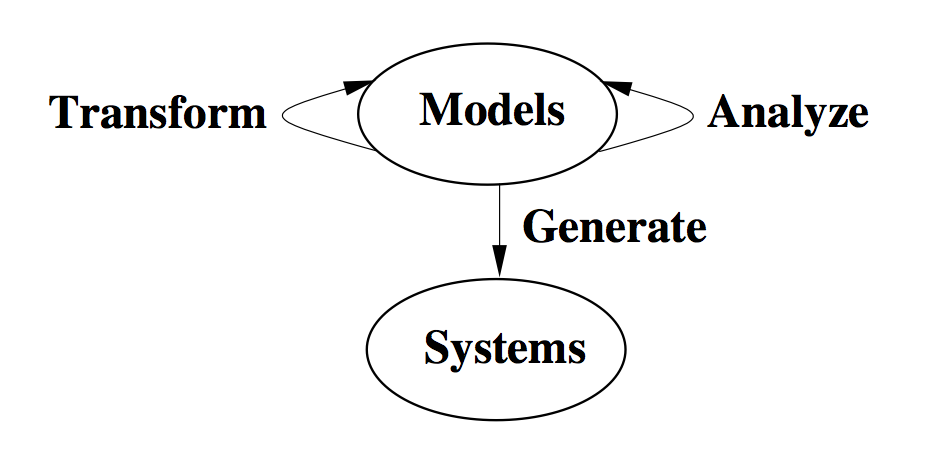
\includegraphics[width=0.6\textwidth]{figura-mdd}
\end{figure}
\bigskip
				
				Sin embargo, códigos de auditoría realizados a los sistemas de votación noruegos
				recomiendan utilizar técnicas de desarrollo relacionadas con el desarrollo basado en pruebas, o
				\textit{Test-Driven Development}, el cual está bien arraigado en varios proyectos 
				open source exitosos, como Spring Framework e Hibernate, y muchos otros proyectos usan
				TDD parcialmente como SQLite o Mono-Project. "Técnicas ya probadas como revisiones de código
				obligatorias, análisis estático, uso de listas para prueba y estándares para documentación y código
				pueden resultar en beneficios de calidad tangibles, así como mejoras en confiabilidad, verificabilidad,
				legibilidad, mantenibilidad, extensibilidad, y otras "-ilidades''.''\cite{Bjørstad2013}

				En términos temporales, se deben establecer ciclos de desarrollo 
				análogos a los correspondientes ciclos electorales. Esto permite entregar prototipos y versiones
				finales del sistema a tiempo para las elecciones, realizar pruebas y experimentos durante
				el período electoral a fin de obtener datos y evidencia para poder conducir el desarrollo del 
				siguiente ciclo de mejor manera. 


%%%%%%%%%%%%%%%%

\begin{table}[h!]
\centering
\caption{Nº de estudios que proponen modelos,esquema o protocolos de e-voting}
\label{tab:estudios-propuestas}
\begin{tabularx}{\textwidth}{X c} 
\toprule[1.5pt]
	%	\bf 			& \bf \\ 
	Estudios que plantean modelos, esquemas o protocolos de e-voting				&	101	\\
	Estudios que incluyen explícitamente requerimientos no funcionales				&	60	\\
	Estudios que presentan modelos que incluyen RNF							&	34	\\	
	Estudios que presentan implementaciones que incluyen RNF					&	6	\\			
\bottomrule[0.5pt]
\end {tabularx}
\end{table}
\bigskip
